% File: algo.tex
% Date: Fri May 03 18:27:32 2013 +0800
% Author: Yuxin Wu <ppwwyyxxc@gmail.com>

\section{Algorithms}
\subsection{Feature Detection}
Lowe's SIFT algorithm is implemented. See \verb|sift.cc, keypoint.cc|.

The algorithm follows the following procedure:
\begin{enumerate}
  \item Build a Scale-Space, which consists of $ S \times O$ grey images.
    The original image is resized in $ O$ different sizes (octaves), and each is then Gaussian-Blured
    by $ S$ different $ \sigma$s.
    \begin{figure}[H]
      \centering
      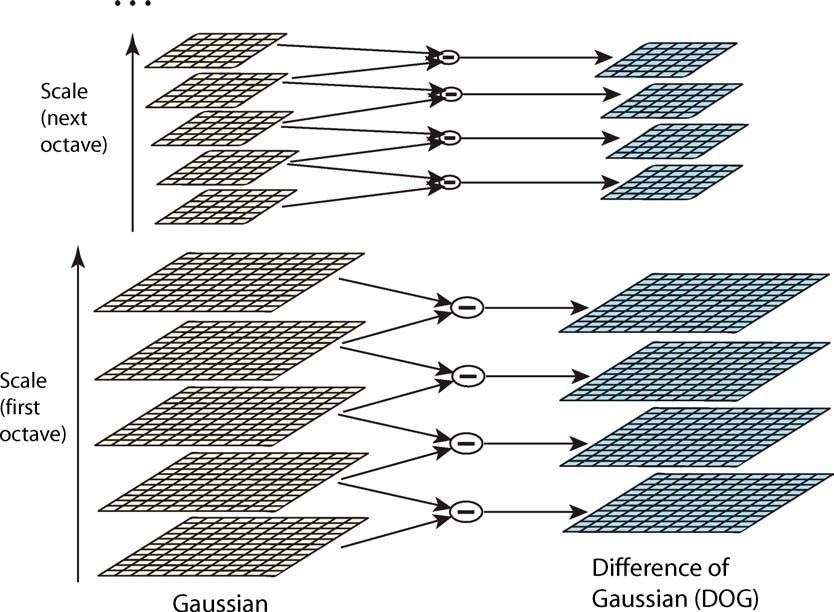
\includegraphics[scale=0.3]{res/dog.png}
      \caption{Scale Space and DOG Space \label{fig:dog}}
    \end{figure}

  \item Build a Difference-of-Gaussian Space.
    In each octave, calculate the differences of every two adjacent blured images.
    Therefore, DOG Space consists of $ (S - 1) \times O$ grey images.
    As shown in \figref{dog}

  \item Detect extrema. In DOG Space, detect all the minimum and maximum
    by comparing a pixel with its 26 neighbors in three directions: $ x, y, \sigma$.
    See \figref{extrema} and \figref{extrema2}
    \begin{figure}[H]
      \begin{minipage}[b]{0.46\linewidth}
        \centering
        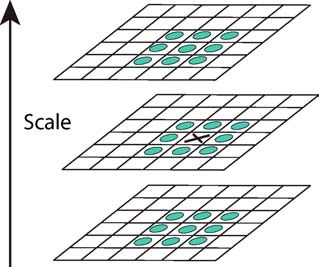
\includegraphics[scale=0.4]{res/extrema.png}
        \caption{Extrema Detection\label{fig:extrema}}
      \end{minipage}
      \hspace{1em}
      \begin{minipage}[b]{0.46\linewidth}
        \centering
        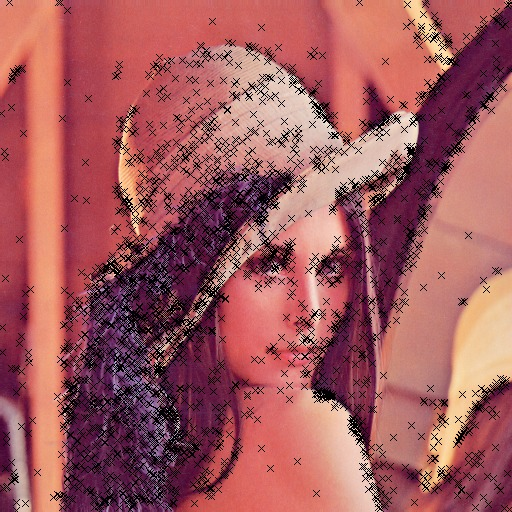
\includegraphics[scale=0.4]{res/extrema_lenna.png}
        \caption{Extrema Example\label{fig:extrema2}}
      \end{minipage}
    \end{figure}

  \item Keypoint Localization.
    Use linear interpolation to calculate offset,
    moving the extrema to a more accurate location.
    Then reject the points with low contrast or on the edge to get true features.
    See \figref{feature1}, \figref{feature2}, \figref{feature3}.
    \begin{figure}[H]
      \begin{minipage}[b]{0.46\linewidth}
        \centering
        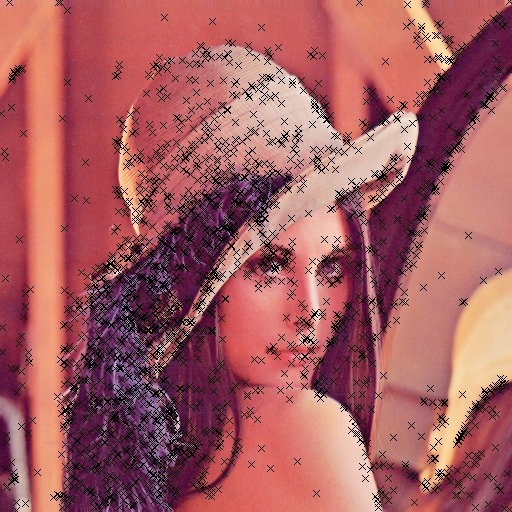
\includegraphics[scale=0.4]{res/feature_after_offset.png}
        \caption{After Localization \label{fig:feature1}}
      \end{minipage}
      \hspace{1em}
      \begin{minipage}[b]{0.46\linewidth}
        \centering
        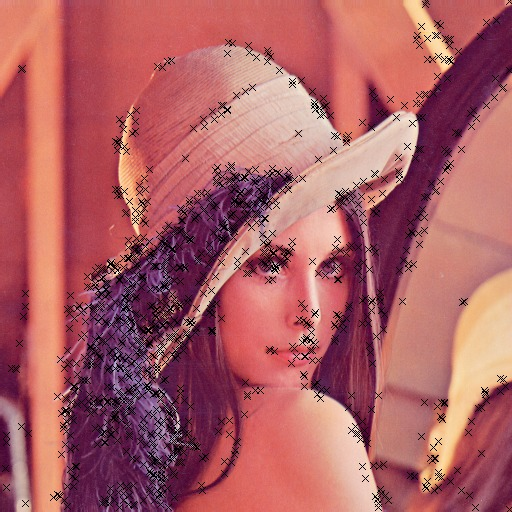
\includegraphics[scale=0.4]{res/feature_after_contrast.png}
        \caption{After Rejecting Low Contrast\label{fig:feature2}}
      \end{minipage}

      \begin{minipage}[b]{0.46\linewidth}
        \centering
        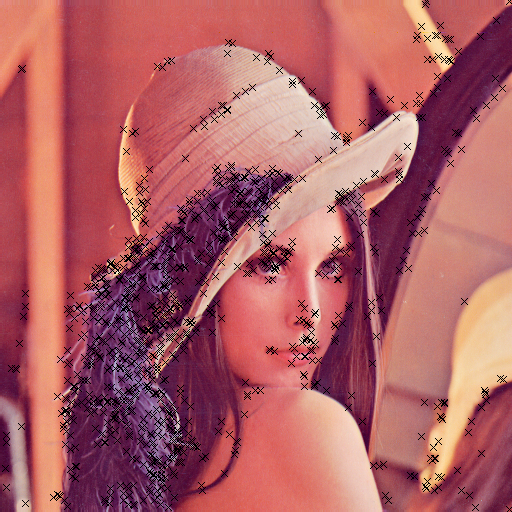
\includegraphics[scale=0.4]{res/feature_point.png}
        \caption{After Eliminating Edge Point\label{fig:feature3}}
      \end{minipage}
      \hspace{1em}
      \begin{minipage}[b]{0.46\linewidth}
        \centering
        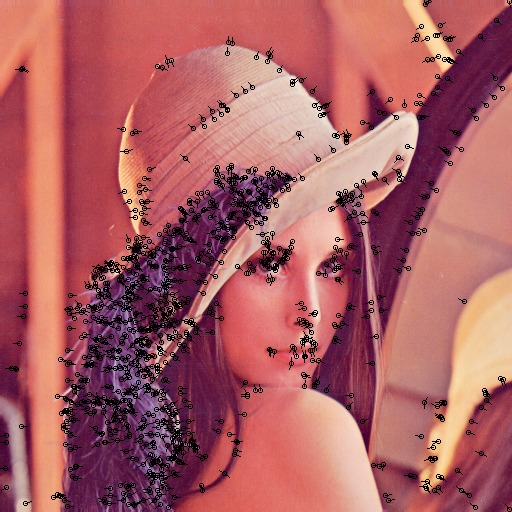
\includegraphics[scale=0.4]{res/feature_dir.png}
        \caption{After Assigning Orientation\label{fig:feature4}}
      \end{minipage}
    \end{figure}

  \item Orientation Assignment.
    We have to first calculated the gradient and orientation of every point in the Scale Space.
    For each keypoint, a histogram of the orientations of its nearby points is built,
    weighted by a gaussian kernel and the magnitude of gradient.
    The peak in the histogram is chosen to be the orientation of the keypoint, as shown by the arrow in \figref{feature4}.

   \item Descriptor Representation.
     Lowe suggest choosing 16 points around the keypoint and building 16 orientation histograms,
     each with 8 different possible values.
     Since all the orientation is relative to the keypoint's orientation,
     this feature is roatation-invariant. The final SIFT feature is a 128-dimensional array.

     \item Feature Matching.
       The Euclidean distance of the 128-dimensional descriptor is the criteria for feature matching between two images.
       A match is considered not convincing and therefore rejected
       if the distances to its closest neighbor and second-closest neighbor are similar.
       The result is shown in \figref{match}.
\begin{figure}[H]
  \centering
  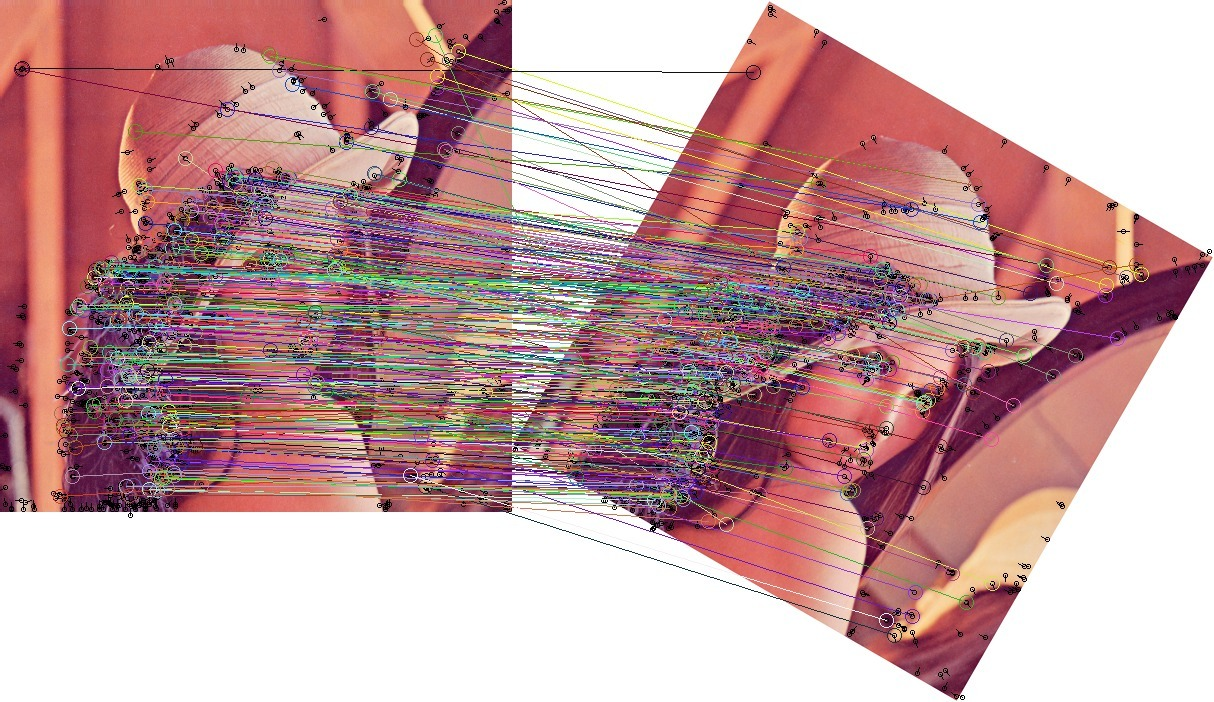
\includegraphics[width=1.0\textwidth]{res/match.png}
  \caption{Matching Result\label{fig:match}}
\end{figure}


\subsection{Warping}
As suggested by a number of literature, a homography transform is needed to match the keypoints.
But a pure homography transform on a planar works
only if the camera moved in pure translation or around a fixed center.

If a panorama input (pure rotation) is given, using homography on a planar leads to vertical distortion, like \figref{distort}.
\begin{figure}[H]
  \centering
  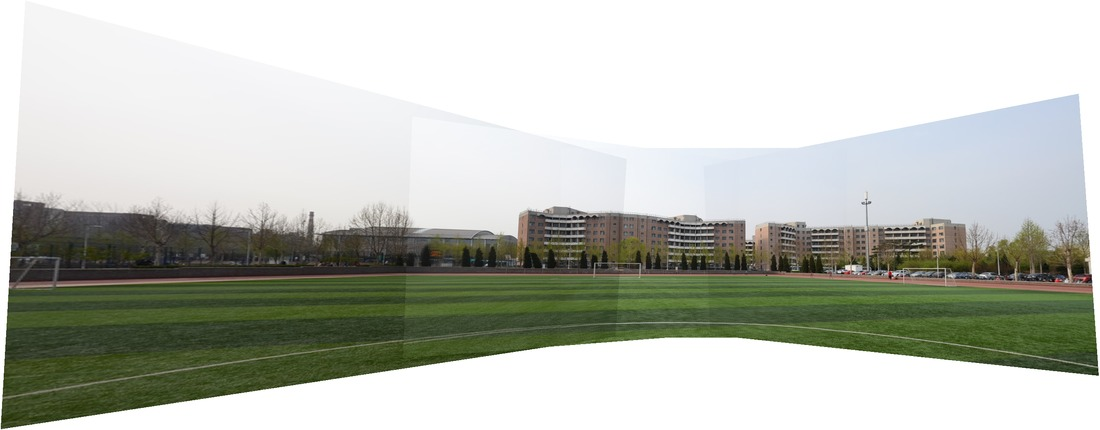
\includegraphics[width=1.0\textwidth]{res/distort.png}
  \caption{Vertical Distortion with Homography on a Planar\label{fig:distort}}
\end{figure}

Therefore, if the option \verb|TRANS = 0|,
every input image as well as the features will be projected to a cylinder before stitching by the following formula:

\[  \begin{cases}
  x' = k\arccos{\dfrac{x}{\sqrt{x^2 + z^2}}}\\
  y' = k\dfrac{y}{\sqrt{x^2 + z^2}}
\end{cases}\]
where $ z$ is chosen to be $ \max\{width, height\}$.  The result is in shown in \figref{cyl}
\begin{figure}[H]
  \centering
  \begin{minipage}[b]{0.24\linewidth}
    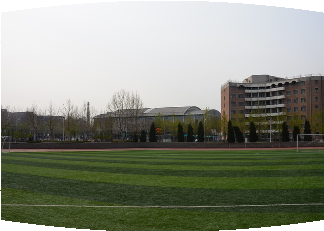
\includegraphics[scale=0.3]{res/1.png}
  \end{minipage}
  \begin{minipage}[b]{0.24\linewidth}
    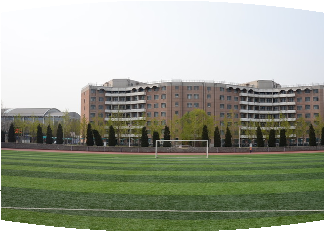
\includegraphics[scale=0.3]{res/2.png}
  \end{minipage}
  \begin{minipage}[b]{0.24\linewidth}
    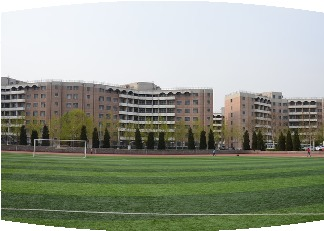
\includegraphics[scale=0.3]{res/3.png}
  \end{minipage}
  \begin{minipage}[b]{0.24\linewidth}
    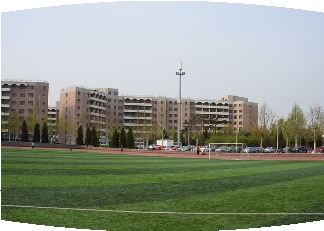
\includegraphics[scale=0.3]{res/4.png}
  \end{minipage}

    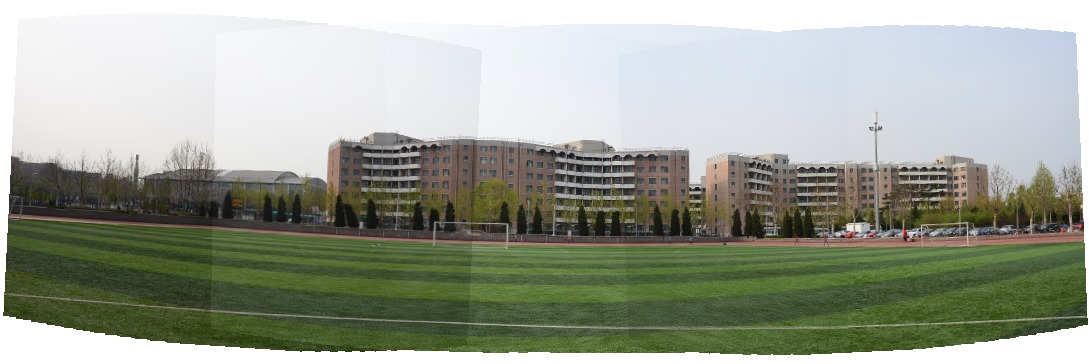
\includegraphics[width=1.0\textwidth]{res/warped_stitch.png}
  \caption{Stitching Result After Projection\label{fig:cyl}}
\end{figure}

\end{enumerate}

\subsection{Transformation}

